\section{Writing Fortran code}

We write a Fortran program that solves Burgers' equation. Instructions for compiling and running the program are located in the README.md file that comes with the source code.

\section{Plotting solutions for sine initial conditions}




\section{Bonus: plotting solutions for square initial conditions}





% \subsection{Creating a Makefile}
%
% We create a Makefile based on the post by a Stackoverflow user Sophie:
%
% \url{https://stackoverflow.com/a/30142139/297131}.
%
% A useful feature of this Makefile is that it places all the build files (*.o, *.mod and executables) into a separate directory called \code{build}. This is, arguably, a better file organization than mixing both the source code and binary  files in the same directory.
%
% Furthermore, we have extended the Makefile by adding ability to create an executable for unit tests by running
%
% \code{\$ make test}
%
% command. This is accomplished by selecting files that have names ending with ``\code{\_test.f90}'' and using them to build the test executable. When the main executable is made, those test source files are excluded.
%
%
% \subsection{Creating \code{Output} module}
%
% We create an \code{Output} module. It contains \code{write\_output} function that writes $x$, $t$ values, as well as the solution 2D array, to a binary data file. The format of the data file is documented in the README.md. We have chosen a binary file instead of a text file because a binary file needs less storage space, and it is faster to read and write.
%
%
% \subsection{Creating \code{Grid} module}
%
% Next, we write a \code{Grid}  module that initializes the arrays for storing x, t and solution values.
%
%
% \subsubsection*{1. Array of $x$ values}
%
% First, we create a 1D array that stores the $x$ values. The range for the $x$ variable is divided into cells of equal size located between $x\_start$ and $x\_end$ numbers. The total number of cells is set by the $nx$ parameter. Parameters $nx$, $x\_start$ and $x\_end$ are supplied to the program by the user. The $x$ values are set to be in the middle of their cells.
%
% For example, suppose we have four x cells, starting from $0$ and ending with $10$, as shown on \autoref{fig_x_grid}. In this case the $x$ array will contains four values: $1.25$, $3.75$, $6.25$ and $8.75$.
%
% \begin{figure}[!ht]
%     \centering
%     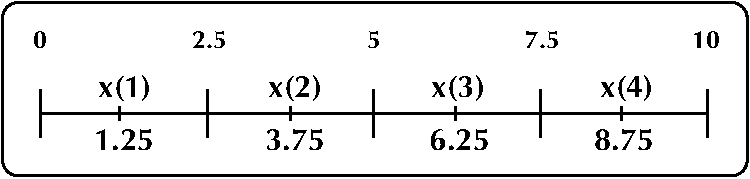
\includegraphics[width=0.8\textwidth]{figures/x_grid.pdf}
%     \caption{Array for storing four x values that are evenly spread in the middle of their cells between zero and ten.}
%     \label{fig_x_grid}
% \end{figure}
%
%
% \subsubsection*{2. Array of $t$ values}
%
% Next, we allocate a 1D array to store the time values. The time values start with $t\_start$ and end with $t\_end$ that are supplied by the user. However, unlike the $x$ values, the number of $t$ values is not supplied by the user, since, in general, the size of the time step can change during calculation. Therefore, we do not yet know the final size of the $t$ array.
%
% This creates a ``chicken and egg'' problem: we need to initialize a $t$ array in order to start calculations, but we do not yet know the size of this array, since it will be determined when calculations are completed. This issue is solved by using an ``allocatable'' keyword that creates a dynamical array, as shown on \code{Line 46} in \autoref{code_initialize_t_array}. On \code{Line 54} we allocate an arbitrary number of $t$ values. Then, later in our program, when we calculate the solution and need to store more $t$ values, we will make the $t$ array larger.
%
% \noindent\begin{minipage}{\linewidth}
% \begin{lstlisting}[caption={Initializing a dynamical array for storing time values (\code{grid.f90}).}, frame=tlrb, numbers=left, firstnumber=46, label={code_initialize_t_array}]
% real(dp), allocatable :: t_points(:)
%
% ! Initial size of the t array, an arbitrary number.
% ! The array will be enlarged when new solutions are calculated.
% nt_allocated = 13
%
% ! Allocate memory for t values.
% allocate(t_points(nt_allocated))
% \end{lstlisting}
% \end{minipage}
%
%
% \subsubsection*{3. Solution array}
%
% Finally, we initialize the most important array that will store the values of the solution. This is a 2D array, its first index is the $x$ dimension, and the second is the time dimension. The array will store the solution for every time iteration. This is not be a good idea if the number of time iterations is very large, since the array may become larger than available memory. However, in our case we use fewer than a thousand time iterations, and consequently the solution array will be small relative to the total memory available.
%
% An example of a solution array is shown on \autoref{fig_solution_array}. Here we create an array for four $x$ values and three $t$ values. In addition, the array contains two extra columns (one on the left and one the right) for storing values of so-called ``ghost'' cells. These are temporary cells that help to make calculation of the solution simpler. These ghost cells will be removed from the solution array when calculations are finished.
%
% \begin{figure}[!ht]
%     \centering
%     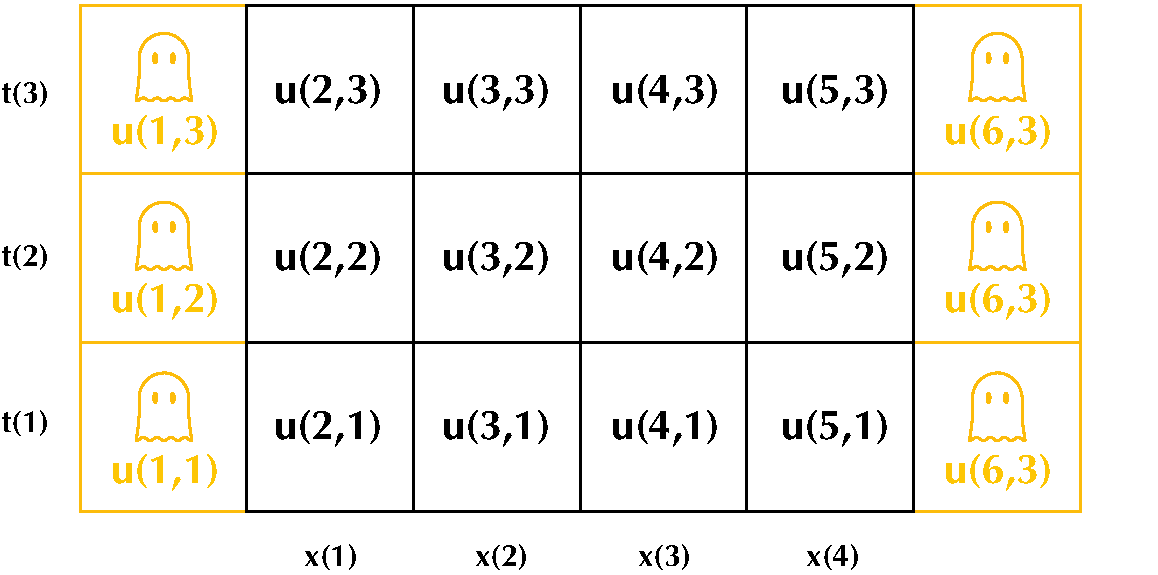
\includegraphics[width=0.8\textwidth]{figures/solution_array.pdf}
%     \caption{An array for storing solution values for four $x$ values and three $t$ values. The array contains two additional columns at the start and the end for storing values for the ``ghost'' cells, which are used for making calculations simpler. }
%     \label{fig_solution_array}
% \end{figure}
%
% The size of the time dimension of the solution array is determined by the number of the $t$ values. Since this number is not known in advance, we use the trick from the time array initialization. Specifically, we create a dynamical  array and allocate its memory using an arbitrary number of time values, as shown in \autoref{code_initialize_solution_array}. Later, as we calculate the solution for growing number of time values, we will resize the solution array and make its time dimension larger.
%
% \noindent\begin{minipage}{\linewidth}
% \begin{lstlisting}[caption={Initializing a dynamical array for storing values of the solution. The $x$ dimension contains two additional columns for storing the ``ghost`` cells. The $y$ dimension has an arbitrary size that will be increased later during calculation to store data for new time values. (\code{grid.f90}).}, frame=tlrb, numbers=left, firstnumber=83, label={code_initialize_solution_array}]
% real(dp), allocatable :: solution(:, :)
%
% allocate(solution(nx + 2, nt_allocated))
% \end{lstlisting}
% \end{minipage}
%
%
% \subsection{Creating \code{InitialConditions} and \code{Step} module}
%
% Next, we create \code{InitialConditions} and \code{Step} modules for calculating initial conditions and performing one step of integration.
%
%
% \section{Implementing Upwind scheme}
%
% We implement Upwind method and solve advection equation
% \[
%   u_t + v \, u_x = 0,
% \]
% with initial condition
% \[
%   u(x, 0) = \sin(2 \pi x),
% \]
% for $x$ from $0$ to $1$. A solution for Upwind scheme are shown on \autoref{fig_sine_c_0_5}.
%
%
% \section{Implementing Lax-Wendroff scheme}
%
% Next, we implement Lax-Wendroff method. Exact and approximate solutions for Lax, Upwind and Lax-Wendroff methods at $t=1 \ s$ are shown on \autoref{fig_sine_c_0_5} and a video is available here:
%
% \texttt{\footnotesize https://youtu.be/zWhv5VOyjhE}
%
% \begin{figure}[!ht]
%     \centering
%     \includegraphics[width=1\textwidth]{figures/{01_sine_c_0.5}.pdf}
%     \vspace*{-5mm}
%     \caption{Exact and approximate solutions to advection equation at $t=1 \ s$ with sine initial conditions and courant factor $C=0.5$.}
%     \label{fig_sine_c_0_5}
% \end{figure}
%
%
% \section{Solutions for square initial conditions}
%
% Next, we solve the equation with square initial conditions. Solutions are shown on \autoref{fig_square_c_0_5} and a video is available here:
%
% \texttt{\footnotesize https://youtu.be/7sHFfG8Rf-A}
%
% \begin{figure}[!ht]
%     \centering
%     \includegraphics[width=1\textwidth]{figures/{02_square_c_0.5}.pdf}
%     \vspace*{-5mm}
%     \caption{Exact and approximate solutions to advection equation at $t=1 \ s$ with square initial conditions and courant factor $C=0.5$.}
%     \label{fig_square_c_0_5}
% \end{figure}
%
%
% \section{Solutions for Courant factor $C=1$}
%
% Next, we use Courant factor $C=1$ instead of $C=0.5$ and solve the equation both with sine and square initial conditions.
%
%
% \subsection{Sine initial conditions}
%
% Solutions for sine initial conditions and $C=1$ are shown on \autoref{fig_sine_c_1} and a video is available here:
%
% \texttt{\footnotesize https://youtu.be/Y47G1ylsle8}
%
% \begin{figure}[H]
%     \centering
%     \includegraphics[width=1\textwidth]{figures/{03_sine_c_1}.pdf}
%     \vspace*{-5mm}
%     \caption{Exact and approximate solutions to advection equation at $t=1 \ s$ with sine initial conditions and courant factor $C=1$.}
%     \label{fig_sine_c_1}
% \end{figure}
%
%
%
% \subsection{Square initial conditions}
%
% Solutions for square initial conditions and $C=1$ are shown on \autoref{fig_square_c_1} and a video is available here:
%
%
% \texttt{\footnotesize https://youtu.be/K3C1n1MkSzQ}
%
% \begin{figure}[H]
%     \centering
%     \includegraphics[width=1\textwidth]{figures/{04_square_c_1}.pdf}
%     \vspace*{-5mm}
%     \caption{Exact and approximate solutions to advection equation at $t=1 \ s$ with square initial conditions and courant factor $C=1$.}
%     \label{fig_square_c_1}
% \end{figure}
%
%
% \section{Analysis of results}
%
% \subsection{Numerical diffusion and dispersion}
%
% We can see from videos
%
% \texttt{\footnotesize https://youtu.be/zWhv5VOyjhE}
%
% and
%
% \texttt{\footnotesize https://youtu.be/7sHFfG8Rf-A}
%
% that solutions from Lax and Upwind methods spread out and deviate from exact solution as time increases. This can be explained by the $\frac{\partial^2 u}{\partial x^2}$ remainder terms in the modified PDEs of the two methods, which produce \emph{numerical diffusion}.
%
% In contrast, Lax-Wendroff method does not have the diffusion term, and we can see that Lax-Wendroff's solution is indistinguishable from exact one for the sine initial conditions (\autoref{fig_sine_c_0_5}). However, the modified PDE of Lax-Wendroff method includes $\frac{\partial^3 u}{\partial x^3}$ term that generates oscillations near discontinuous regions (also known as \emph{numerical dispersion}), which can be seen on video
%
% \texttt{\footnotesize https://youtu.be/7sHFfG8Rf-A}
%
%
% \subsection{Exact solutions for Courant factor $C=1$}
%
% We can see from Figures \ref{fig_sine_c_1} and \ref{fig_square_c_1} that solutions from all three methods are indistinguishable from exact ones for both sine and square initial conditions. This happens probably because the error terms in the modified PDEs of the methods include factors like $(1 - C)$ and $(1 - C^2)$. Consequently, the error terms vanish for $C=1$ and approximate solutions become exact.
%
%
%
